\chapter{Tření}
\label{chap:drag}

O třecích jevech při otáčení spinneru jsme si již byli schopni udělat představu při úvodním kvalitativním sledování. Tření bude hrát značnou roli v našem systému, protože právě tření bude hlavním limitujícím faktorem průběhu chaotického chování. Dalším využitím, kromě našeho hlavního záměru - zpřesnění popisu chování, bude také například možnost odhadnutí maximálního času, než systém ztratí všechnu svou energii. Zajímavým a snadno měřitelným pro nás bude průběh úhlové rychlosti $\omega$ v čase (resp. změna úhlové rychlosti \footnote{$I\dot{\omega} = \tau$}), ze kterého vyplývá i náš popis těchto třecích složek.

Zajímá-li nás tedy změna rychlosti, dovolíme si odhadnout, že hlavními zdroji tření bude ložisko a odpor vzduchu. Provedeme idealizaci ložiska a řekneme, že jeho brzdný moment síly, a tím pádem i úhlové zpomalení, bude neměnné v čase a nezávislé na rychlosti. Toto nemusí být vždy pravda - například objeví-li se v reálném ložisku nějaké nechtěnné oscilace (které jsme sledovali) nebo je-li na ložisko působeno nějakou externí silou mířící kolmo na osu otáčením (jako například když se od sebe velmi silně odpuzují magnety ze dvou blízkých spinnerů). Oba tyto příklady jsou příliš složité k popsání a nejsme je tedy schopni zkoumat. Toto brzdné úhlové zrychlení (resp. zpomalení) nezávislé na rychlosti spinneru označíme $\alpha$.

Další výraznou složkou bude již zmíněný odpor vzduchu. Z látky středoškolské fyziky známe přibližnou úměrnost odporové síly na kvadrátu rychlosti ($F \propto v^2$) při turbulentním proudění (které v našem případě očekáváme kvůli složité geometrii spinneru). Při rotaci spinneru bychom tedy analogicky očekávali proporcionalitu $\dot{\omega} \propto \omega^2$. Míru této závislosti označíme $\gamma$.

Poslední složkou, pro kterou nejsme schopni najít fyzikální podstatu, ale kterou přesto budeme zkoumat je lineární složka $\beta$. Existují-li tedy jevy, které nám unikly, a platí pro ně závislost $\dot{\omega} \propto \omega$, můžeme je kompenzovat touto složkou. Zároveň budeme podrobně srovnávat přesnosti našich předpokladů včetně, ale i bez, této složky, abychom určili, zda dává smysl tuto složku využívat.

\clearpage

\section{Analytický popis}

Všechny tři dříve zmíněné složky dohromady tedy popisuje řídící závislost systému: \footnote{Záporná znaménka používáme čistě z toho důvodu, aby nám koeficienty $\alpha$, $\beta$ a $\gamma$ vycházely kladně, jelikož očekáváme, že systém bude zpomalovat.}:
\begin{equation}
    \label{eq:drag_diff_wlin}
    \dot{\omega}(t) = - \alpha - \beta \omega(t) - \gamma \omega^2(t)
\end{equation}

Pokud bychom odstranili lineární komponent, získáváme:
\begin{equation}
    \label{eq:drag_diff}
    \dot{\omega}(t) = - \alpha - \gamma \omega^2(t)
\end{equation}

Obě tyto diferencialní rovnice jsou analyticky řešitelné a jejich řešení pro $\omega$ jsou v totožném pořadí \footnote{Všimněme si, že rovnice \ref{eq:drag_res_wlin} je ekvivalentní rovnici \ref{eq:drag_res}, když $\beta = 0$.}:
\begin{equation}
    \label{eq:drag_res_wlin}
    \omega(t) = -\frac{\sqrt{4\alpha\gamma - \beta^2} \tan{(\frac{1}{2}\sqrt{4\alpha\gamma - \beta^2}(t-c_1)})-\beta}{2\gamma}
\end{equation}
a
\begin{equation}
    \label{eq:drag_res}
    \omega(t) = -\sqrt{\frac{\alpha}{\gamma}} \tan{(\sqrt{\alpha\gamma}(t-c_1))}
\end{equation}

\subsection{Maximální doba otáčení}

Parametr $c_1$ \footnote{Někdy také označujeme $t_{max}$.} je hodnota v sekundách, která odpovídá době, po které se spinner zastaví. Vyjádřením $c_1$ (např. z druhé rovnice) jsme schopni určit poměrně přesně, jak dlouho se bude spinner točit, známe-li jeho parametry $\alpha$, ($\beta$) a $\gamma$ a jeho počáteční úhlovou rychlost $\omega_0$:
\begin{equation}
    \label{eq:runtime_from_omeg0}
    c_1(\omega_0) = \frac{1}{\sqrt{\alpha\gamma}} \arctan{ \bigg( \sqrt{\frac{\gamma}{\alpha}} \omega_0 \bigg)}
\end{equation}

Pokud bychom si přáli vyjádřit celkovou dobu otáčení z počáteční kinetické energie, můžeme dosadit $E_k = \frac{1}{2}I\omega^2$, kde je nám $I$ již známé (viz \autoref{sec:moment_of_inertia}), a jednoduchou úpravou získáváme:
\begin{equation}
    \label{eq:runtime_from_ene}
    c_1(E) = \frac{1}{\sqrt{\alpha\gamma}} \arctan{ \bigg( \sqrt{\frac{2 \gamma E}{\alpha I}} \bigg)}
\end{equation}

Jakmile dojde k tomu, že $t > c_1$, nepopisuje již funkce náš spinner, protože by začal opět nabývat energii a otáčet se opačným směrem, k čemuž nemůže dojít.

\clearpage

\subsubsection{Horní limit doby otáčení $n$ spinnerů}

Další zajímavou vlastností, kterou jsme schopni pro tento idealizovaný systém dokázat je, že máme-li libovolné (přirozené) množství spinnerů o počátečních energiích $E_1, E_2 ... E_n$, které spolu neinteragují, je maximální dobou $t_{max}$, po kterou se může některý z nich otáčet $t_{max} \leq c_1(\sum_{i=1}^n E_i)$. Tento fakt se může zdát triviálním a zbytečným, ale tímto způsobem jsme schopni určit například horní časovou hranici, po kterou by musela běžet simulace, než bychom si byli poměrně \footnote{Nemůžeme si být kompletně jisti kvůli interakcím spinnerů a nepřestnostem simulace.} jisti, že již došlo k zastavení všech spinnerů.

Pokud bychom chtěli zlepšit tento odhad i pro interagující spinnery, bylo by potřeba počítat s tím, že spinnery se mohou zrychlovat, zpomalovat a často budou oscilovat. Pokud bychom sledovali mnoho přibližně harmonických oscilací spinnerů, kdy se po relativně dlouhou dobu nepohybují svou nejvyšší rychlostí, mohli bychom se inspirovat efektivní hodnotou sinusoidy a udělat tak hrubý odhad, že $t_{max} \leq \sqrt{2} c_1(\sum_{i=1}^n E_i)$. Nad tím, jaká konstanta by byla dobrá, můžeme dlouze polemizovat, ale to není zájmem této práce, proto nebudeme myšlenku dále rozvádět.

Tuto vložku zakončíme důkazem dříve vyslovené věty, že $t_{max} \leq c_1(\sum_{i=1}^n E_i)$:

Nejdříve zdůrazníme několik zřejmých skutečností o naší funkci $c_1(E)$:

\begin{equation}
    \label{eq:max_runtime_proof_p1}
    \begin{gathered}
        c_1(E) = \frac{1}{\sqrt{\alpha\gamma}} \arctan{ \bigg( \sqrt{\frac{2 \gamma E}{\alpha I}} \bigg)} \\
        c_1(E) \text{ je rostoucí a prostá funkce pro } \alpha, \gamma \in \mathbb{R}^+ \\
        E_1, E_2, ..., E_n \in \mathbb{R}^+ \implies c_1(E_1), ..., c_1(E_n) \in \mathbb{R}^+
    \end{gathered}
\end{equation}

Bez újmy na obecnosti poté můžeme řící, že:
\begin{equation}
    \label{eq:max_runtime_proof_p2}
    \begin{gathered}
        E_1 \leq E_2 \leq ... \leq E_n \in \mathbb{R}^+ \implies c_1(E_1) \leq ... \leq c_1(E_n) \in \mathbb{R}^+
    \end{gathered}
\end{equation}

A obecně vybereme energie $E_u$ a $E_v$ takové, že $E_u \geq E_v$ ($u \neq v \wedge 1 \leq v < u \leq n$), pro které se snažíme dokázat následující:

\begin{equation}
    \label{eq:max_runtime_proof_p3}
    \begin{gathered}
        c_1(E_u+E_v) \stackrel{?}{\geq} \max(c_1(E_u), c_1(E_v)) \\
    \end{gathered}
\end{equation}

\clearpage

\subsubsection{Důkaz}
\begin{equation}
    \label{eq:max_runtime_proof_p4}
    \begin{gathered}
        c_1(E_u+E_v) \geq \max(c_1(E_u), c_1(E_v)) \\
        \\
        c_1(E_u+E_v) \geq \max(c_1(E_u), c_1(E_v)) \equiv c_1(E_u+E_v) \geq c_1(E_u) \because (c_1(E_u)\geq c_1(E_v) \because E_u \geq E_v) \\
        \\
        c_1(E_u+E_v) \geq c_1(E_u) \\
        \frac{1}{\sqrt{\alpha\gamma}} \arctan{ \bigg( \sqrt{\frac{2 \gamma (E_u+E_v)}{\alpha I}} \bigg)} \geq \frac{1}{\sqrt{\alpha\gamma}} \arctan{ \bigg( \sqrt{\frac{2 \gamma E_u}{\alpha I}} \bigg)} \\
        \arctan{ \bigg( \sqrt{\frac{2 \gamma (E_u+E_v)}{\alpha I}} \bigg)} \geq \arctan{ \bigg( \sqrt{\frac{2 \gamma E_u}{\alpha I}} \bigg)} \\
        \sqrt{\frac{2 \gamma (E_u+E_v)}{\alpha I}} \geq \sqrt{\frac{2 \gamma E_u}{\alpha I}}\\
        \sqrt{\frac{2 \gamma }{\alpha I}} \sqrt{E_u+E_v} \geq \sqrt{\frac{2 \gamma}{\alpha I}} \sqrt{E_u}\\
        \sqrt{E_u+E_v} \geq \sqrt{E_u}\\
        E_u+E_v \geq E_u\\
        E_v \geq 0\\
        \text{QED}
    \end{gathered}
\end{equation}

Dále pouhou analogií pro libovolné dvojice, větší $k$-tice a konečně celou $n$-tici energií je zřejmé, že:
\begin{equation}
    \label{eq:max_runtime_proof_p5}
    \begin{gathered}
        \forall E_j; (1 \leq j \leq n): c_1(E_j) \leq c_1 \Bigg(\sum_{i=1}^n E_i \Bigg) \\
        \Updownarrow \\
        t_{max} \leq c_1 \Bigg(\sum_{i=1}^n E_i \Bigg) \\
        \text{QED}
    \end{gathered}
\end{equation}

\subsection{Určení jednotek parametrů $\alpha$, $\beta$ a $\gamma$}

Přepsáním rovnice \ref{eq:drag_diff_wlin} pouze pomocí jednotek jsme schopni jednoduše odvodit jednotky koeficientů $\alpha$, $\beta$ a $\gamma$:
\begin{equation}
    \label{eq:drag_units}
    \begin{gathered}
        [rad \cdot s^{-2}] = - [\alpha] - [\beta] [rad \cdot s{-1}] - [\gamma] [rad \cdot s]^2 \\
        [rad \cdot s^{-2}] = - [rad \cdot s^{-2}] - [s^{-1}] [rad \cdot s{-1}] - [rad^{-1}] [rad^2 \cdot s^{-2}] \\
        \implies [\alpha] = [rad \cdot s^{-2}]; [\beta] = [s^{-1}]; [\gamma] = [rad^{-1}]
    \end{gathered}
\end{equation}

\clearpage

\subsection{Experiment pro potvrzení analytického řešení}

Abychom ověřili, zda výsledky našich diferencialních rovnic odpovídají realitě, provedeme měření, kde budeme sledovat jak se snižuje úhlová rychlost každého z našich spinnerů v čase. K tomu využijeme opět magnetického čidla Vernier MG-BTA, které bude sledovat momenty, kdy se kolem něj mihne jeden z magnetů připevněných na ramenou spinneru (velmi podobně jako u \autoref{fig:spinner_pendulum_aparature}). Časová hustota těchto vrcholů je úměrná úhlové rychlosti - přesněji 1 vrchol za sekundu se rovná $\frac{2}{3}\pi$ $rad/s$.

\begin{wrapfigure}{r}{0.5\textwidth}
    \vspace*{-1.5cm}
    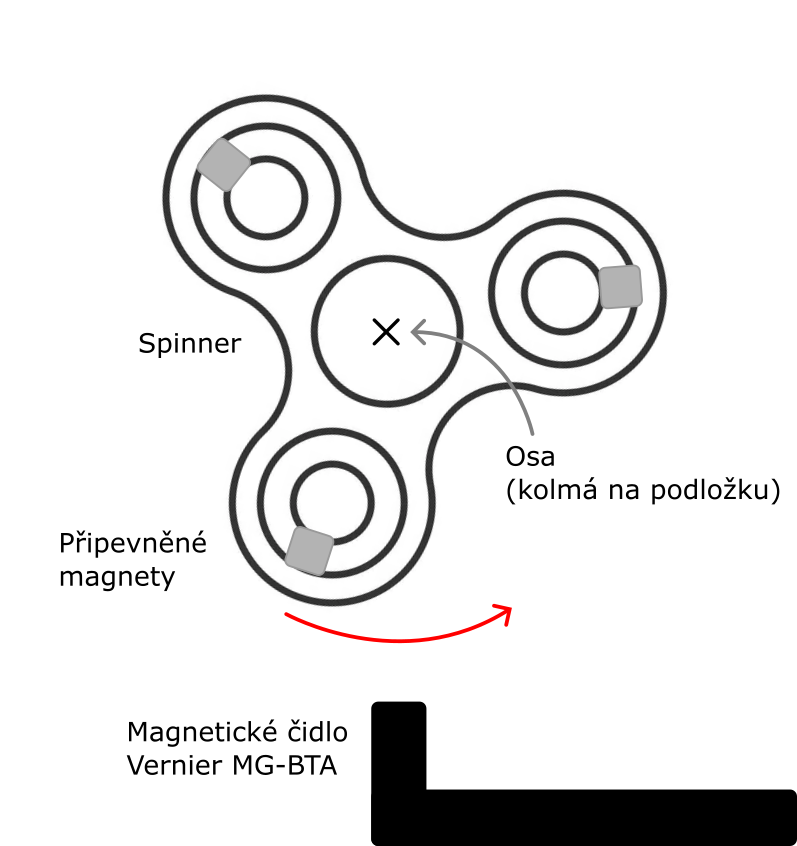
\includegraphics[width=0.45\textwidth]{drag_setup.png}
    \centering
    \caption{Ilustrace aparatury pro měření přibližné úhlové rychlosti spinneru}
    \label{fig:spinner_drag_aparature}
\end{wrapfigure}

\subsubsection{Aparatura}
Aparatura tohoto experimetu (vyobrazená na \autoref{fig:spinner_drag_aparature}) je velmi podobná té na \autoref{fig:spinner_pendulum_aparature}. Jediným rozdílem je, že nyní má spinner osazená všechna ramena a to pouze jedním magentem. Zároveň není zavěšen ve své ose, ale leží na podložce a je tedy jeho osa otáčení kolmá na prodložku (resp. rovnoběžná se směrem gravitačního zrychlení). V této orientaci budou prováděna i všechna následující měření v dalších kapitolách.

\begin{wrapfigure}{r}{0.5\textwidth}
    \vspace*{3cm}
    \includegraphics[width=0.5\textwidth]{peak_find_alg_drawing.png}
    \centering
    \caption{Ilustrace fungování algoritmu pro hledání peaků}
    \label{fig:peak_find_alg_drawing}
\end{wrapfigure}
\subsubsection{Zpracování dat}
Ke zpracování dat opět použijeme jazyk \texttt{Python} a stejné knihovny jako doposud.
Prvním úkolem je převedení průběhů kmitů magnetického pole (způsobených mihnutím magnetu před čidlem) do průběhu úhlové rychlosti v čase.
K tomto bude potřeba určit peaky a jejich pozici v čase a následně konvolucí počítat množství peaků na určitých intervalech.
Pozice peaků určíme tak, že budeme sledovat kdy naměřená hodnota překročí nějaký práh. Toto bude začátek našeho peaku.
Když půjde zpět pod hodnotu prahu, ukončíme peak. Pozici maxima umístíme do středu tohoto časového intervalu (viz \autoref{fig:peak_find_alg_drawing}).

\clearpage
\lstinputlisting[language=Python, caption=Kód k hledání pozic peaků, label=code:3]{./prilohy/snippets/c3.py}
Druhým krokem je projít celou časovou domému měření a rozdělit ji na menší intervaly. V těchto intervalech spočítáme počet peaků a přepočtem $1$ $peak/s = \frac{2\pi}{3}$ $rad/s$ určíme přibližnou průměrnou rychlost v tomto okolí.

\clearpage
\lstinputlisting[language=Python, caption=Pokračování kódu \ref{code:3} - výpočet úhlové rychlosti pomocí konvoluce, label=code:4]{./prilohy/snippets/c4.py}

\subsection{Výsledky a porovnání se simulací}
Po analýze všech naměřených dat výše uvedeným algorimem (celkem 7 měření, protože máme 7 různých spinnerů) a provedením fitu funkcí dle rovnice \ref{eq:drag_res_wlin} získáváme koeficienty v následucících rozmezích:
\begin{equation}
    \label{eq:drag_coef_res}
    \begin{gathered}
        0.220 \leq \alpha \leq 0.927 \\
        0.0 \cdot 10^{-15} \leq \beta \leq 2.5 \cdot 10^{-3} \\
        2.22 \cdot 10^{-4} \leq \gamma \leq 3.17 \cdot 10^{-4} \\
    \end{gathered}
\end{equation}

\subsection{Zhodnocení použití lineárního koeficientu}

\begin{wrapfigure}{r}{0.6\textwidth}
    \vspace*{0cm}
    \includegraphics[width=0.6\textwidth]{spinner_decay_with_beta.png}
    \centering
    \caption[Příklad grafu měřeného průběhu $\omega$ v $t$ s $\beta \neq 0$]{Příklad grafu měřeného průběhu úhlové rychlosti v čase (zeleně) v porovnání s fitem užívajícím všech tří brzdných složek (červeně). Simulace modře.}
    \label{fig:drag_fit_wlin}
\end{wrapfigure}

Nyní je na řadě prozkoumání významu a užitečnosti lineárního brzdného koeficientu. Získané hodnoty $\beta$ z předchozích sedmi měření nejsou konzistetní mezi spinnery, což je prvním indikátorem toho, že lineární složka nebude součástí dobrého popisu tření (alespoň pro tento případ).

Fitujeme-li stejná data funkcí bez lineární složky získáváme graf \ref{fig:drag_fit}. Vidíme, že simulace (jejíž implementací se budeme zabývat v \autoref{chap:sim}) v tomto případě lépe předpovídá měřené hodnoty.
\begin{wrapfigure}{r}{1\textwidth}
    \includegraphics[width=1\textwidth]{spinner_decay.png}
    \centering
    \caption[Příklad grafu měřeného průběhu $\omega$ v $t$ s $\beta = 0$]{Příklad grafu měřeného průběhu úhlové rychlosti v čase (zeleně) v porovnání s fitem užívajícím pouze složek $\alpha$ a $\gamma$ (červeně). Simulace modře.}
    \label{fig:drag_fit}
\end{wrapfigure}

\clearpage

Poslední měření, které jsme k účelům porovnání těchto dvou metod provedli, bylo sledování průběhu úhlové rychlosti, když byl spinner umístěn do magnetického pole našeho velkého magnetu. Velký magnet jsme upevnili 8cm od středu spinneru a stejnou aparaturou jako v minulém experimentu jsme sledovali jeho chování. Zde jsme prováděli pouze jedno měření a fitovali jsme ho opět oběma způsoby, které porovnáváme níže:
\begin{figure}[H]
    \includegraphics[width=0.65\textwidth]{sim_spinner_magnetic_with_beta.png}
    \centering
    \caption[Příklad grafu měřeného průběhu $\omega$ v $t$ s $\beta \neq 0$ v magnetickém poli]{Graf měřeného úhlové rychlosti v čase v porovnání s fitem užívajícím všech tří složek. (barevné schéma jako v \autoref{fig:drag_fit_wlin})}
    \label{fig:drag_fit_mag_wlin}
\end{figure}
Jak můžeme vidět na \autoref{fig:drag_fit_mag_wlin}, koeficient $\beta$ nám vychází efektivně nulový a průběhy fitů, ani simulací, se od sebe téměř neliší.
Z těchto měření tedy ověřujeme naši předchozí představu, že lineární komponent tření není fyzikálně signifikantní.
\begin{figure}[H]
    \includegraphics[width=0.65\textwidth]{sim_spinner_magnetic.png}
    \centering
    \caption[Příklad grafu měřeného průběhu $\omega$ v $t$ s $\beta = 0$ v magnetickém poli]{Graf měřeného úhlové rychlosti v čase v porovnání s fitem užívajícím složek $\alpha$ a $\gamma$. (barevné schéma jako v \autoref{fig:drag_fit})}
    \label{fig:drag_fit_mag}
\end{figure}
